\documentclass[conference]{IEEEtran}
\usepackage{subcaption}
\usepackage{caption}
\hyphenation{op-tical net-works semi-conduc-tor}
\usepackage{amsmath,amssymb,graphicx}
\usepackage{tablefootnote}
\usepackage{textcomp}
\makeatletter
\setlength{\@fptop}{0pt}
\makeatother
\renewcommand{\figurename}{Figure}
\setlength{\textfloatsep}{6pt}
\def\IEEEbibitemsep{0pt plus .5pt}
\begin{document}
%
% paper title
% can use linebreaks \\ within to get better formatting as desired
\title{A Comparison of Antenna Placement Algorithms\vspace{-3ex}}

\author{\IEEEauthorblockN{Abhinav Jauhri}
\IEEEauthorblockA{Carnegie Mellon University\\
ajauhri@cmu.edu}}
\maketitle
\begin{abstract}
%\boldmath
Co-location of multiple antenna systems on a single fixed or mobile platform can be challenging due to a variety of factors, such as mutual coupling, individual antenna constraints, multipath, obstructions, and parasitic effects due to the platform. The situation frequently arises where a new communication capability, and hence antenna system, is needed on an existing platform. The problem of placing new antennas requires a long, manual effort in order to complete an antenna placement study. An automated procedure for determining such placements would not only save time, but would be able to optimize the performance of all co-located antenna systems. In this work, we examine a set of stochastic algorithms to determine their effectiveness at finding optimum placements for multiple antennas on a platform. To our knowledge, this is the first study to investigate optimizing multiple antenna placement on a single platform using multiple stochastic algorithms. Of the four algorithms compared on the basis of convergence rates, simulated annealing and evolutionary strategy were found to be most effective in finding optimum placements.
\end{abstract}
% IEEEtran.cls defaults to using nonbold math in the Abstract.
% This preserves the distinction between vectors and scalars. However,
% if the conference you are submitting to favors bold math in the abstract,
% then you can use LaTeX's standard command \boldmath at the very start
% of the abstract to achieve this. Many IEEE journals/conferences frown on
% math in the abstract anyway.

% no keywords

% For peer review papers, you can put extra information on the cover
% page as needed:
% \ifCLASSOPTIONpeerreview
% \begin{center} \bfseries EDICS Category: 3-BBND \end{center}
% \fi
%
% For peerreview papers, this IEEEtran command inserts a page break and
% creates the second title. It will be ignored for other modes.
\IEEEpeerreviewmaketitle



\section{Introduction}
Antenna placement on a multi-antenna platform currently involves a manual process that is challenging, time consuming, and may result in sub-optimum placements leading to low communication system performance. Moreover, the search space is highly complex and becomes exponentially large with the number of antennas to be placed ($|\text{search space}| = m^n$, where $m$ is the number of allowable placements for each antenna and $n$ is number of antennas). 

Stochastic optimization techniques have been used extensively for non-convex and non-linear search spaces to avoid sub-optimum results due to the multimodal nature of the search space (see figure \ref{fig:tc1_ss}). Applying Evolutionary Algorithms (EA), a type of stochastic optimization technique, to the antenna placement problem could help determine placements which increase the effectiveness of each antenna. Evolutionary algorithms encompass a variety of computer search technologies, the Genetic Algorithm (GA) being the most well-known. Moreover, EAs have been proven capable in discovering high performance antenna designs deployed in space \cite{lohn2005evolutionary}. 

In this work, we have analyzed stochastic algorithms to help determine optimum or near-optimum antenna placements on a platform. The problem has been modeled and simulated using antenna modeling software package called NEC2. The approach does not depend on the specifications of antennas, and platforms. The algorithmic-set includes Genetic Algorithm, Evolutionary Strategy, Simulated Annealing, and Hill Climbing.

\section{Related Work}
\label{sec:related}
The problem of optimizing the placement of multiple antennas on a single platform has rarely been studied.  The closest research concerns algorithms for locating and configuring infrastructure for cellular wireless networks with the assumption of isotropic radiation pattern \cite{rais2005}. Another related work computes optimum antenna locations restricted to a mobile device. In our work, none of the algorithms utilize prior information on good antenna placements or type of antennas, but depend on allowable placement of antennas on the given platform.

The related problem of co-designing antennas for a given platform ({\em in-situ} design) using stochastic algorithms has been investigated in \cite{linden2000wire} with encouraging results. Because antenna placement bears many similarities to antenna design, we believe that stochastic algorithms will prove effective.

\section{Problem Formulation}
\label{sec:problem}
\subsection{Inputs}
\label{sec:inputs}
A platform for placing multiple antennas could vary from a simple rectangular box to an aircraft. Our inputs to an algorithm comprise of a platform and set of antennas each with allowable placements on the platform. Formally, a platform, $P$, is defined in 3-dimensional space with its surface discretized into a regular grid with some spacing consisting of potential antenna placement points. Let $n$ denote the number of antennas to be placed on $P$ such that $n>1$, and $A$ represent the set of antennas: $A = \{A_1, ..., A_n\}$. For each antenna $A_i$, $L_i$ denote the set allowable placement coordinates $\in \mathbb R^3$ on $P$ such that the size of $\mid L_i \mid =m_i$, and $ \forall i, m_i>1$:
\[
L_i = \{(x_{1}, y_{1}, z_{1}), ..., (x_{m_i}, y_{m_i}, z_{m_i})\}
\]
For example, figure \ref{fig:tc1_figure} has $n=2$ and $m=84$ for each antenna.
\begin{figure}%
    \begin{subfigure}{\columnwidth}
        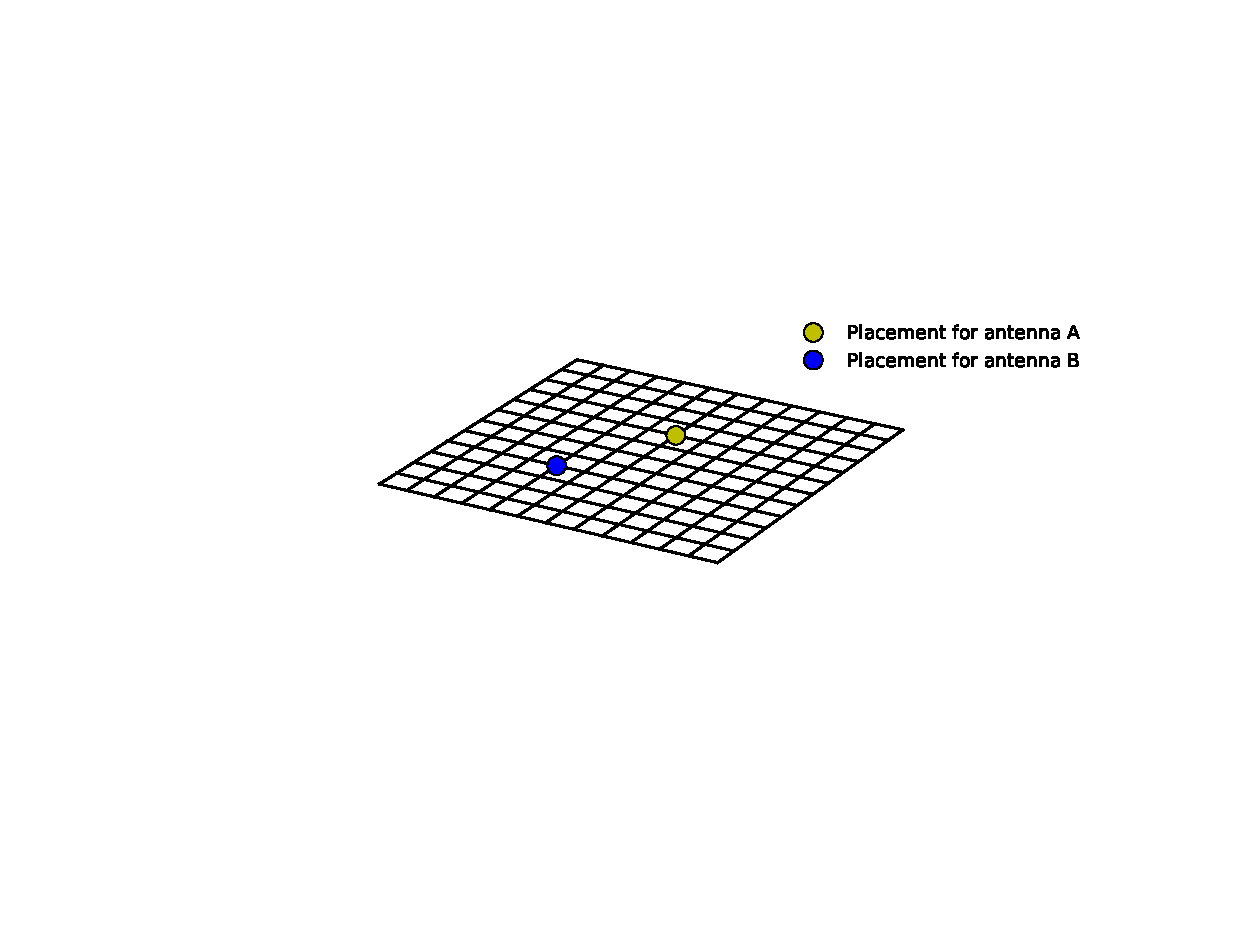
\includegraphics[width=\columnwidth]{FIG/tc1_reco2}%
    \end{subfigure}\hfill\\
    \caption{Search space for test case 1, having multiple local optimum solutions shown in shades of blue.}%
    \label{fig:tc1_ss}%
\end{figure}

Using the allowable placements ($L_i$), a \textit{candidate solution} or \textit{individual} is a placement configuration of $n$ antenna locations, one for each of the $n$ antennas, in 3-dimensional space:
\[
    \text{Candidate Solution}  = \left\{l_i | l_i \in L_i, i \in [1,n]\right\}
\]
Candidate solutions are the building blocks for each algorithm we evaluate the antenna placement problem on. It is important to note that the number of allowable placements for any antenna are finite. 

\subsection{Fitness Evaluation}
The stochastic algorithms used to optimize the placement of antennas find the best candidate solution such that the radiation pattern and mutual coupling are optimum. For radiation pattern, we minimize the difference between the free-space gain pattern (FSG) of each antenna $A_i$, and its in-situ gain (ISG) pattern when placed on a platform along with other antennas. Minimizing the difference from the free-space gain pattern will ensure better communication capability. For each antenna $A_i$ we compute multiple field points around an antenna:

\begin{equation} \label{eq:rp}
    F_{RP} = \sum_{i=1}^n\sum_{\theta=0}^\pi\sum_{\phi=0}^{2\pi}
           \left| FSG_i(\theta,\phi) - ISG_i(\theta,\phi) \right| ^2,
\end{equation}
where $\theta$ \& $\phi$ define the spherical coordinates of a field point.

For the second objective, it is desired to minimize the mutual coupling between two antennas to reduce the overall energy loss. This is computed in a pairwise manner where the $CP$ function computes the coupling between two antennas:
\begin{equation}
  F_{MC} = \sum_{i=1}^{n-1}\sum_{j=i+1}^{n} CP(A_i, A_j)
\end{equation}

The overall objective is to find a candidate solution which minimizes the fitness value $F$, defined as:
\begin{equation} \label{eq:optimal}
  F = \alpha F_{MC} + \beta F_{RP},
\end{equation}
where $\alpha$ and $\beta$ are constants such that $\alpha + \beta = 1$. 

Radiation pattern and antenna coupling are measured in decibels (dB) which is a logarithmic unit used to express the ratio between two quantities. For radiation pattern parameter, the \textit{antenna strength} or \textit{gain} shown in Eq.\eqref{eq:rp}, at any given point on a sphere defined by $(\theta, \phi)$ is the ratio of the signal strength of the antenna being tested and a perfectly isotropic antenna. For coupling, the ratio compares the energy absorbed by an antenna when another antenna is operating nearby. Coupling reduces antenna efficiency, and is undesirable for the multiple antenna placement problem.

\section{Stochastic Search Algorithms}
\label{sec:algorithms}
%\begin{itemize}
%    \item A hypothesis used by any algorithm is similar to as defined in the previous Section \ref{sec:inputs}.
%    \item For any hypothesis, no two antenna placements overlap. It may be the case that two different antennas have overlapping set of allowable placements, but the formation of any hypothesis avoids such a case as it may result in imprecise calculation of fitness.
%    \item The $fitness(H)$ function used in all four algorithms is the equivalent of Eq.\eqref{eq:optimal}, assuming we have its inputs i.e. $F_{MC}$ and $F_{RP}$.
%\end{itemize}
\subsection{Genetic Algorithm}
\label{sec:algorithms-ga}
Genetic algorithm is the simplest of all evolutionary algorithms which aim to model Darwinian evolution and natural selection to evolve a population of candidate solutions. They have been used extensively as stochastic search procedures for numerous applications \cite{fogel1994}.

Evolution operators in our version of GA are \textit{one-point crossover} and \textit{uniform mutation}. For one-point crossover operation, two individuals are selected with one being uniformly chosen from the population and the other from a tournament selection. For all experiments, crossover probability was $60\%$ and mutation probability as $10\%$. Intuitively, a high mutation probability drives the algorithm into a random search and renders the evolutionary aspect of the algorithm weak. The size of the individual is not arbitrarily large, and therefore it was preferred to restrict the mutation such that only one antenna placement was manipulated. Since we have a discrete set of placements (end points of wires of a platform), mutation step size renders a new placement from the set of allowable placements. This mutation operator is similar for all other algorithms as well.

For arbitrarily large number of antennas, one may consider changing the mutation operator to manipulate more than one antenna placement. 
\subsection{Evolutionary Strategy}
\label{sec:algorithms-es}
The evolutionary strategy $(\mu + \lambda)$ is different from a genetic algorithm in the following ways: 
mutation is the primary operator here for maintaining diversity in the population since there are no crossover operations. Survivor selection is performed by choosing fittest $\mu$ individuals that are included in the next generation. $1:7$ ratio was maintained between $\mu$ and $\lambda$. 

For mutation of an individual, both the antenna and its new placement are selected uniformly at random from the allowable placements. We ensure that there is no overlap with any other antenna defining the individual during the mutation. ES is more effective than GA since the mutation operator is applied multiple times on the same individual ($\lambda$ times on each of the $\mu$ individuals). Preservation of the best $\mu$ individuals helps the algorithm to maintain more diversification in the population, making the search more useful.
\subsection{Simulated Annealing}
\label{sec:algoriths-sa}
Simulated annealing is a local search algorithm with a neighborhood structure. The algorithm moves from one individual to one of its neighbours in accordance to a probabilistic criterion. If the fitness improves then the neighbouring individual is accepted. Otherwise, the move is accepted only with a probability depending on fitness change and control parameter called temperature. Probability is given by: $exp( \frac{\Delta fitness}{T_i})$. This helps the algorithm to escape local optimum solutions in a multimodal search space. We used a linear cooling schedule for temperature $T_i = \tau T_{i-1}$ with $\tau = f(m_{iters})$. Due to different sizes of the search space, cooling schedule is a function of the maximum iterations ($m_{iters}$), which are approximately $50\%$ of the total allowable placements. The initial temperature for SA range $\in [0.23, 0.27]$.
\subsection{Hill Climbing}
\label{sec:algoriths-hc}
Hill climbing is a greedy search algorithm different from simulated annealing as there is no temperature cooling schedule. This property and its greedy nature of accepting only fitter individuals make HC prone to getting stuck with locally optimum solutions. However, the ease of implementation and effectiveness in numerous optimization problems \cite{skalak1994} makes hill climber a popular approach for optimization.

\section{Experimental Setup}
\label{sec:setup}
We used an open source antenna modeling software called Numerical Electromagnetic Code (NEC2) to calculate the fitness of an individual. NEC2 provides a convenient interface to input details about the platform with mounted antennas, and to collect simulation results. Possible antenna locations are written as a set of wires with a start point and end point in 3-dimensional space.

All test cases describe platforms which are replicas of real-world use cases like mobile devices, tanks, and cars. Antennas used on these platforms are used extensively in contemporary microwave systems. Figure \ref{fig:tc_figures} shows all test cases used for our experiments. Table \ref{tab:tcs} shows the allowable number of placements for each antenna used in different test cases. 
\begin{figure}
    \centering
    \begin{subfigure}{.5\columnwidth}
        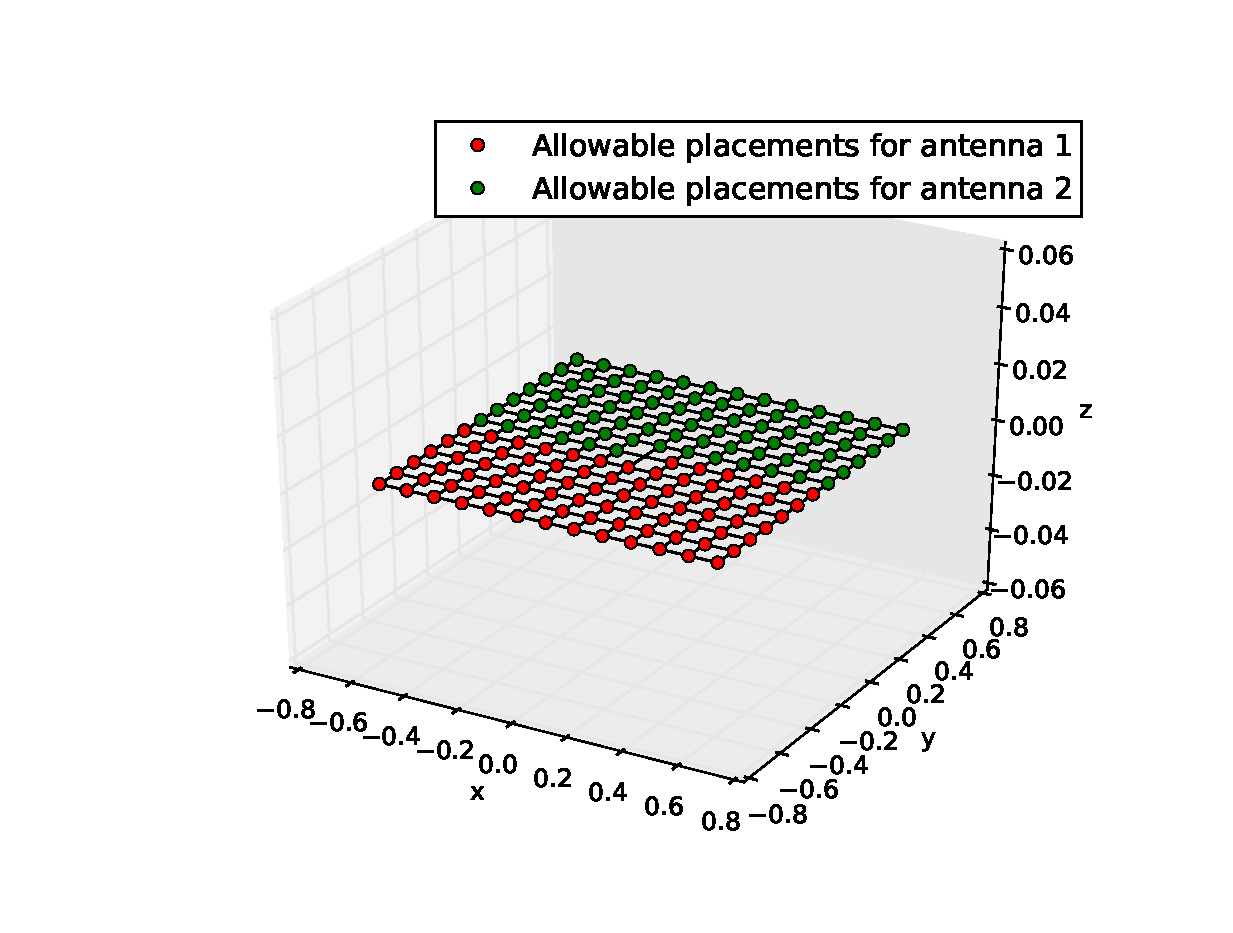
\includegraphics[width=\columnwidth,height=\columnwidth]{FIG/tc1_figure}%
        \caption{Test Case 1}%
    \label{fig:tc1_figure}%
    \end{subfigure}\hfill%
    \begin{subfigure}{.5\columnwidth}
        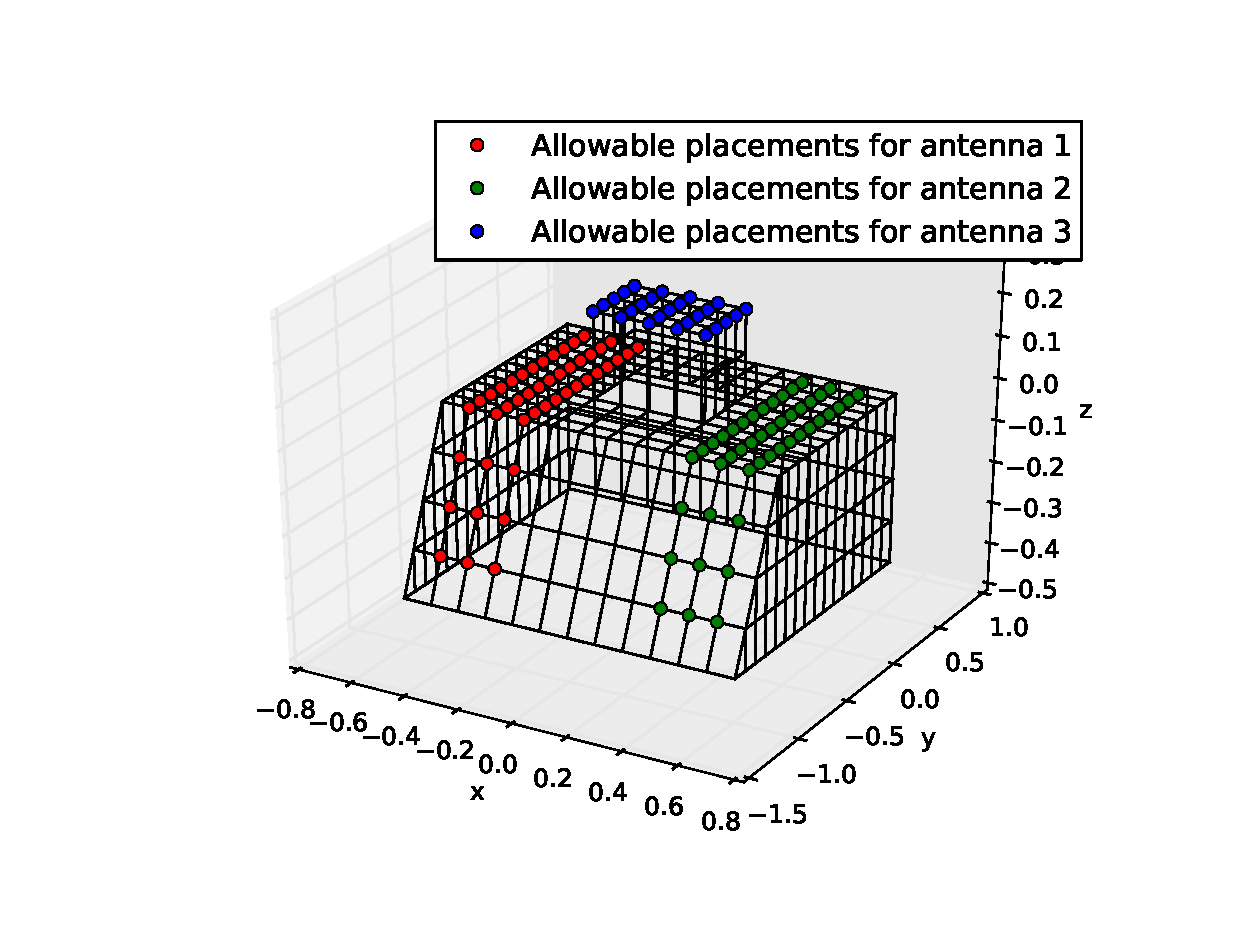
\includegraphics[width=\columnwidth, height=\columnwidth]{FIG/tc2_figure}%
        \caption{Test Case 2}%
    \label{fig:tc2_figure}%
    \end{subfigure}\hfill\\%
    \begin{subfigure}{.5\columnwidth}
        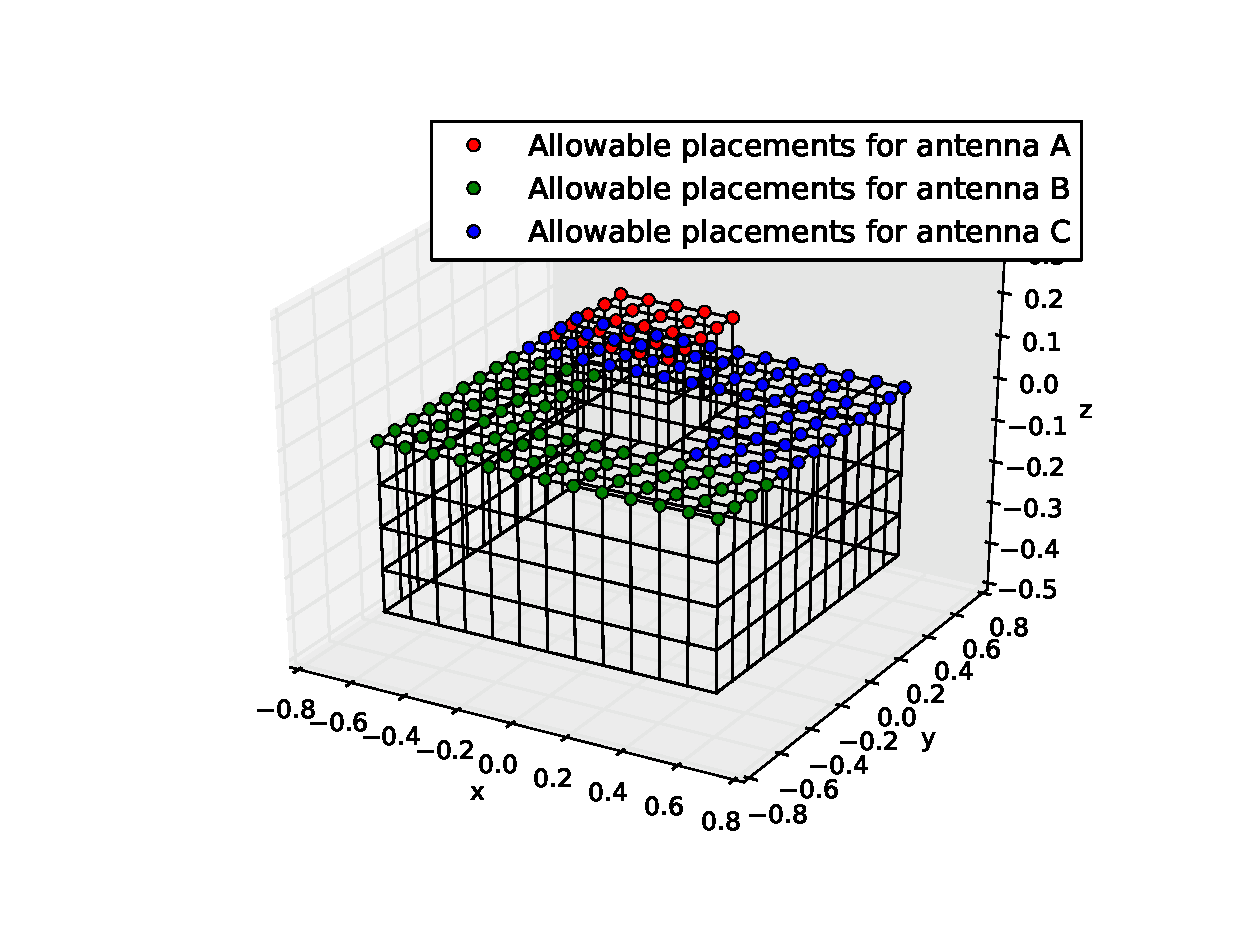
\includegraphics[width=\columnwidth, height=\columnwidth]{FIG/tc3_figure}%
        \caption{Test Case 3}%
    \label{fig:plat2}%
    \end{subfigure}\hfill%
    \begin{subfigure}{.5\columnwidth}
        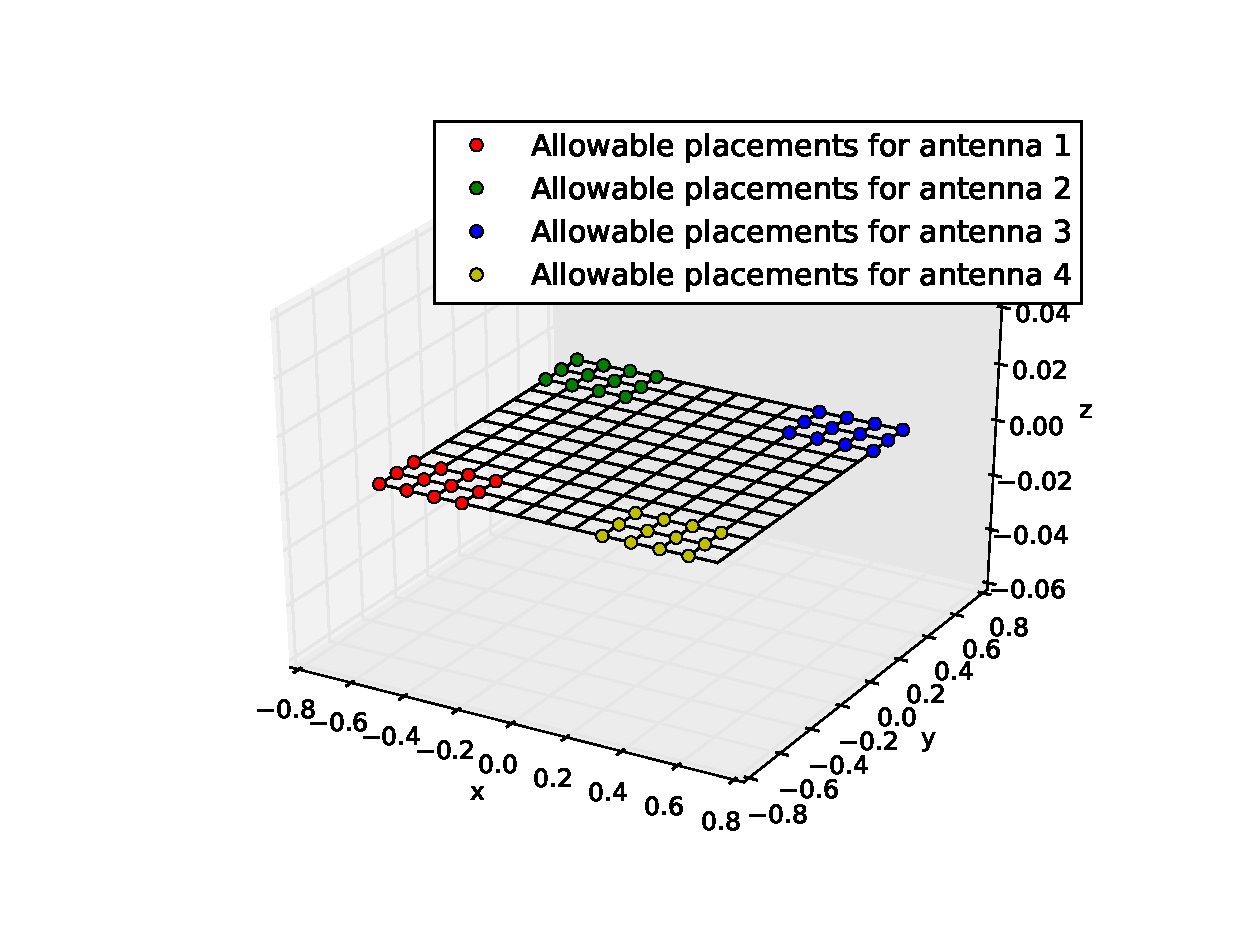
\includegraphics[width=\columnwidth,height=\columnwidth]{FIG/tc4_figure}%
        \caption{Test Case 4}%
        \label{fig:plat3}%
    \end{subfigure}\hfill
    \caption{Antennas and platforms for $4$ test cases used}
    \label{fig:tc_figures}
\end{figure}

\begin{table}
\centering
\caption{Antenna Placement Test Cases} \label{tab:tcs}
\begin{tabular}{|c|c|c|} \hline
    Test Case&Number of Antennas&Number of allowable placements\tablefootnote{Allowable placements for each antenna are provided within parenthesis}\\ \hline
1 & 2 & 7,056 (84x84) \\ \hline
2 & 3 & 50,625 (45x45x25) \\ \hline
3 & 3 & 126,025 (71x71x25) \\ \hline
4 & 4 & 20,736 (12x12x12x12) \\
\hline\end{tabular}
\end{table}

 
For radiation pattern, the number of field points is determined by the product of total number of unique $\theta$ and $\phi$ values which encompass points in a sphere around the antenna. All experiments computed the radiation gain over $4140$ points with increments of $4$\textdegree $~$ for $\theta$ and $\phi$. For all test cases antennas were excited with the same frequency of $100$ MegaHertz.

For fitness evaluation of a candidate solution, input files are generated with all specifications of antennas and the platform. NEC2 would use the input files to generate radiation pattern values for all pairs of $(\theta, \phi)$. Similarly, for the second fitness parameter - mutual coupling, NEC2 provides results between all possible pairs of antennas. If $n=4$, then there are $\binom{4}{2}$ pairs for which mutual coupling is calculated.

Each test case was first evaluated with an exhaustive search algorithm to determine an optimum fitness value, and its corresponding candidate solution from the entire search space. The results from the exhaustive search were also used to normalize fitness function values between $[0,1]$. For all experiments $\alpha = \beta = 0.5$ in Eq.\eqref{eq:optimal}. The termination criteria for a run of an algorithm was either the global minimum or $0.5 \cdot \left|S\right|$, where $\left|S\right|$ is the size of the search space. The criterion was determined as half of the search space as most of the algorithms had stagnated their search as visible from plots in figure \ref{fig:tc_mf}.

\section{Simulation Results}
\label{sec:results}
Genetic Algorithm (GA) and Evolutionary Strategy (ES) operate on a population of candidate solutions at any given iteration as oppose to Simulated Annealing (SA) and Hill Climbing (HC) which operate on one candidate solution. For this reason the mean best fitness in figure \ref{fig:tc_mf} is higher in the initial stages of a run for SA and HC than GA and ES, because in a population there is higher probability of creating a fitter individual. In terms of computational time of any algorithm, the bottleneck is the running time of NEC2 simulator. Therefore, the mean best fitness is shown against the percentage of fitness evaluations which is equivalent to the number of runs of NEC2 simulator. In all four test cases, the best candidate solution was found by ES in less than $25\%$ fitness evaluations of the search space. 

Regions in the plot where the mean best fitness of GA and ES is constant relates to the fitness evaluation of offsprings created by evolutionary operators applied on the population of candidate solutions. For SA and HC, we notice the SA curve crossing the HC curve in all four test cases. This is due to the temperature parameter of SA, allowing it to accept fitness worsening individuals with high probability initially in the run. However, later in the run the cooling schedule reduces the probability of SA accepting a worse individual. Eventually, SA has a better probability to reach the optimum solution in comparison to HC.

As known in general, the HC algorithm made progress only in the initial phases of the run and got stuck in local optimums. The purpose for inclusion of such a random search algorithm was to highlight that antenna placement may not always be a trivial optimization task as can be seen from the search space figure \ref{fig:tc1_ss}. The search space for test case 4 always had a lower fitness candidate solution in the neighbourhood, therefore allowing HC to converge quickly.

To summarize, figure \ref{fig:tc_mf} shows that ES was successful in finding optimum candidate solutions for all test cases. Alternatively, SA took less number of fitness evaluations to converge but had a lower probability in finding the optimum solution.
\begin{figure*}
    \centering
    \begin{subfigure}{\columnwidth}
        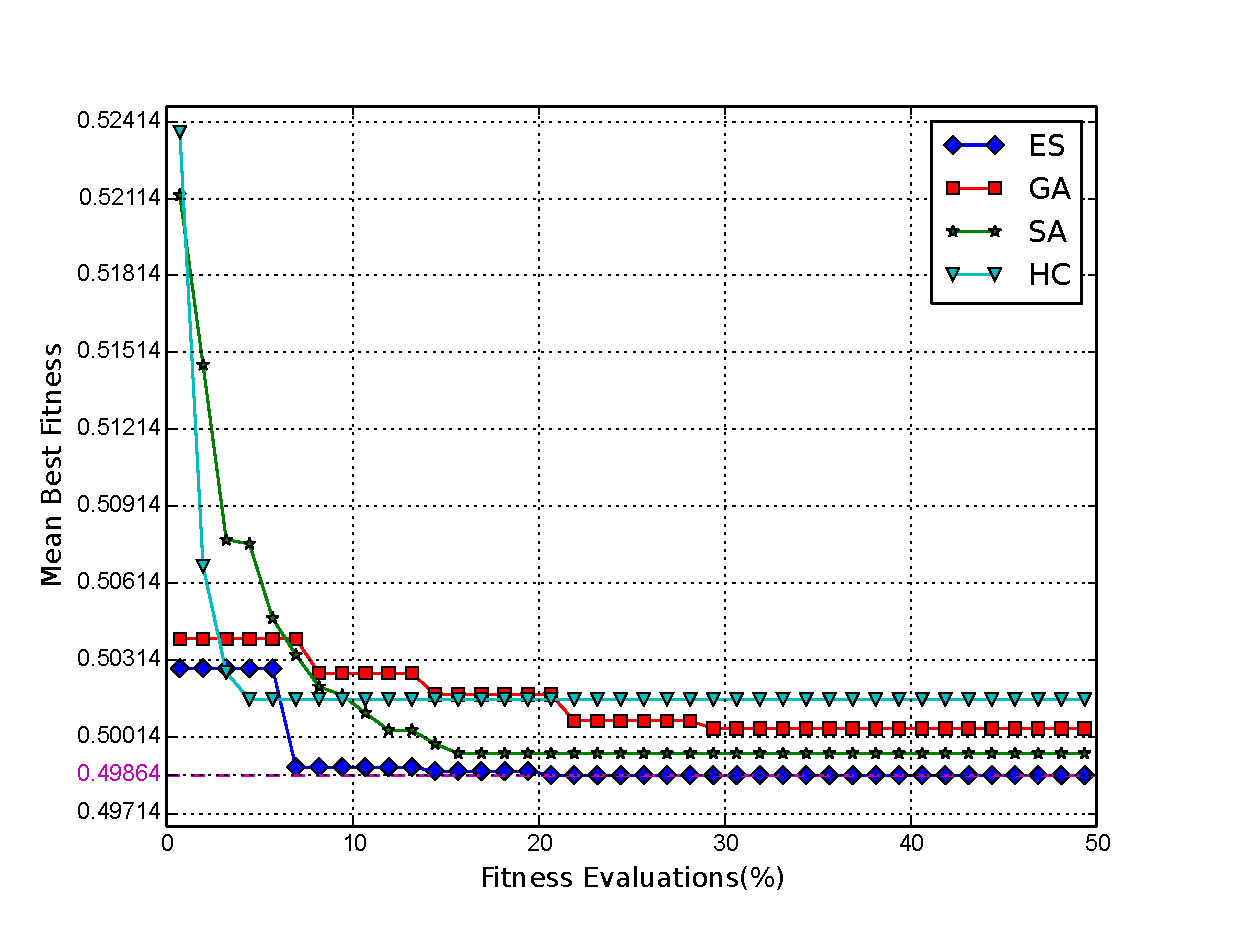
\includegraphics[width=\columnwidth]{FIG/tc1_mf.eps}%
        \caption{Test Case 1}%
    \label{fig:tc1_mf}%
    \end{subfigure}\hfill%
    \begin{subfigure}{\columnwidth}
        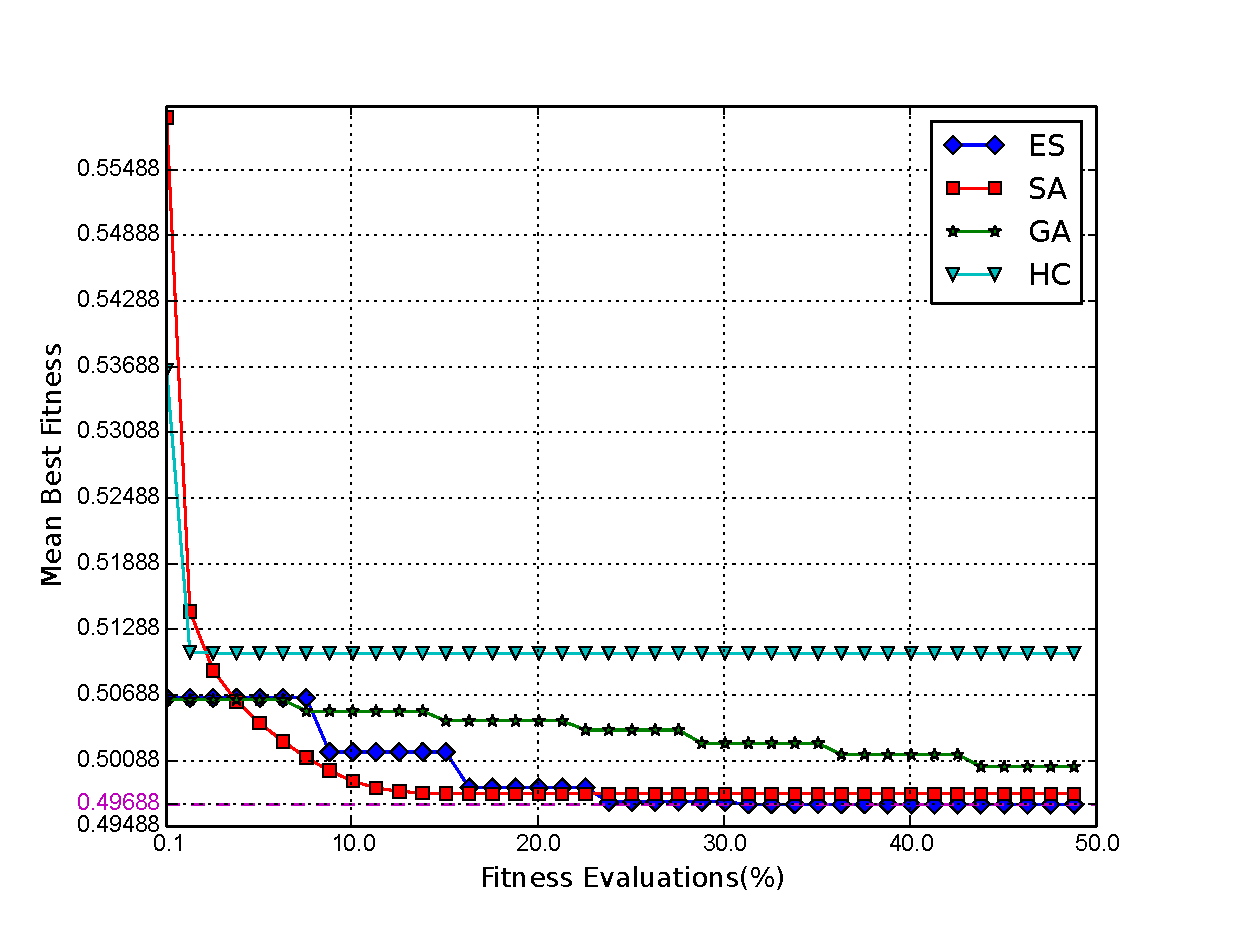
\includegraphics[width=\columnwidth]{FIG/tc2_mf.eps}%
        \caption{Test Case 2}%
        \label{fig:tc2_mf}%
    \end{subfigure}\hfill\\
    \begin{subfigure}{\columnwidth}
        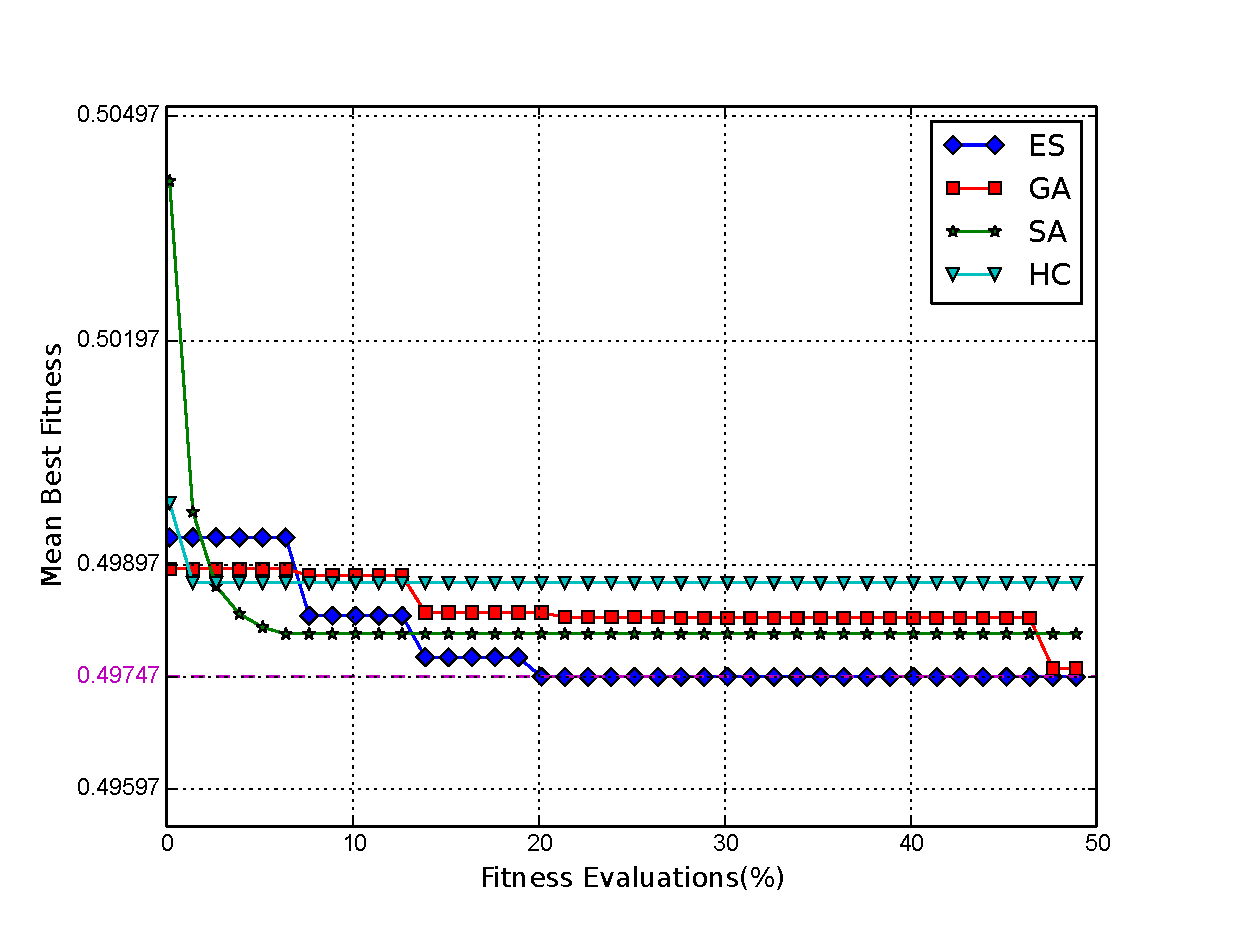
\includegraphics[width=\columnwidth]{FIG/tc3_mf.eps}%
        \caption{Test Case 3}%
        \label{fig:tc3_mf}%
    \end{subfigure}\hfill%
    \begin{subfigure}{\columnwidth}
        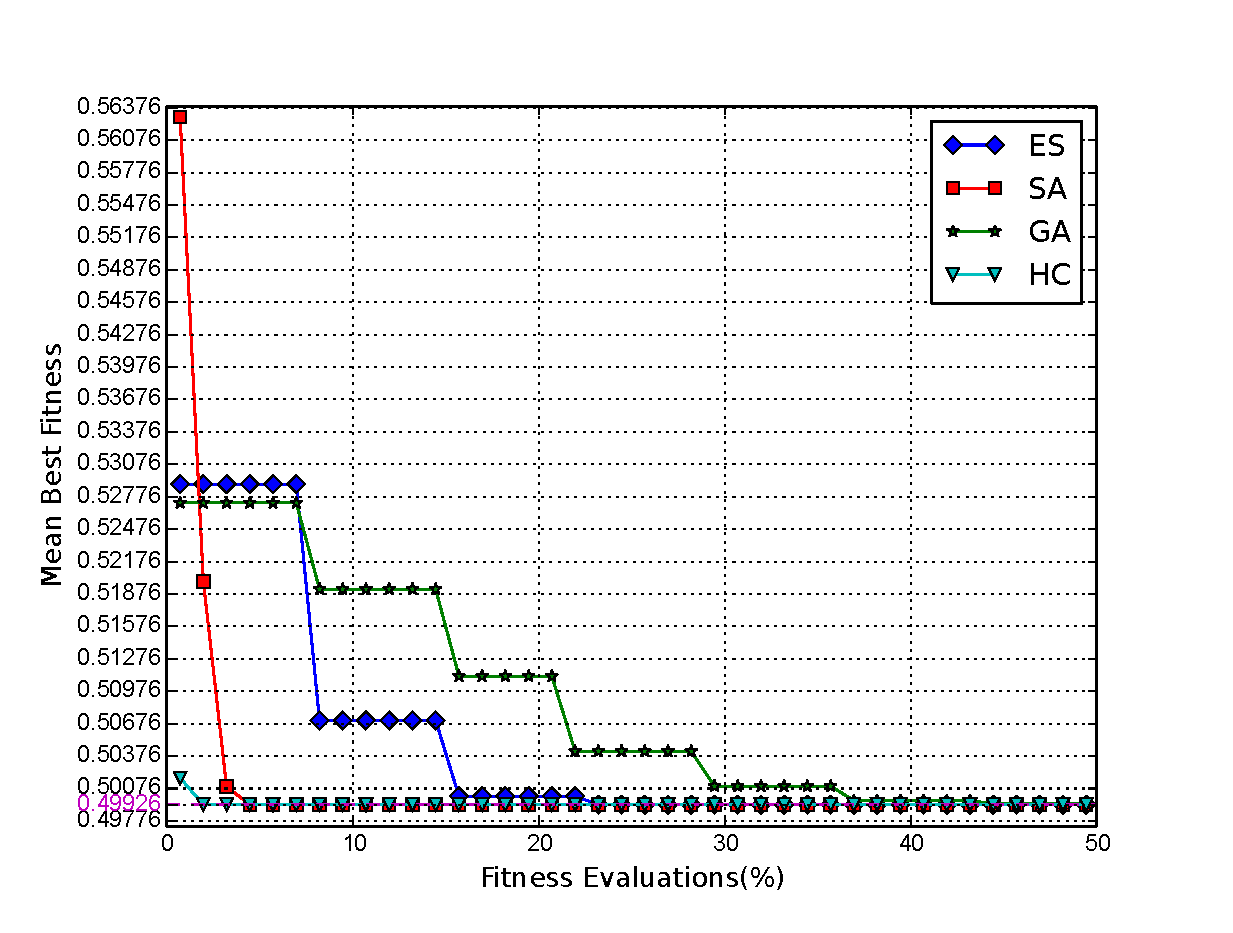
\includegraphics[width=\columnwidth]{FIG/tc4_mf.eps}%
        \caption{Test Case 4}%
        \label{fig:tc4_mf}%
    \end{subfigure}\hfill%
    \caption{Mean best fitness shown for $10$ independent runs of each algorithm for $4$ test cases. Global minimum calculated using exhaustive search algorithm for each test case shown in magenta on the vertical axis. The horizontal axis is representative of the percentage of fitness evaluations of the search space. The number of evaluations may not be unique points in the search space.}
\label{fig:tc_mf}
\end{figure*}
 

\section{Conclusion \& Future Work}
In this paper, a comparison of four stochastic algorithms applied to antenna placement optimization problem has been presented. The results show that a trade-off space exists: faster, less successful search by SA versus slower, more successful search by ES. GA was not very effective, and slower in finding the optimum individual. More importantly, our formulation is generic such that it can be applied to any type of a platform which otherwise may be time consuming and expensive in case of large objects like satellites, warships, and aircrafts. 

Most of the stochastic algorithms presented here were elementary. More experiments can be conducted for population based algorithms with different population sizes, to statistically compare how this may affect the performance of the algorithm. Also, bigger search spaces need to be considered with more number of antennas. Other evolutionary techniques like ALPS, and Differential Evolution can also be compared for quality and convergence.

\begin{thebibliography}{1}

\bibitem{lohn2005evolutionary}
Lohn, Jason D., et al. ``Evolutionary design of a single-wire circularly-polarized x-band antenna for nasa's space technology 5 mission.'' Antennas and Propagation Society International Symposium, 2005 IEEE. Vol. 2. IEEE, 2005.

\bibitem{linden2000wire}
Linden, Derek S. "Wire antennas optimized in the presence of satellite structures using genetic algorithms." Aerospace Conference Proceedings, 2000 IEEE. Vol. 5. IEEE, 2000.

\bibitem{fogel1994}
Fogel, David B. "An introduction to simulated evolutionary optimization." Neural Networks, IEEE Transactions on 5.1 (1994): 3-14.

\bibitem{skalak1994}
Skalak, David B. "Prototype and feature selection by sampling and random mutation hill climbing algorithms." Proceedings of the eleventh international conference on machine learning. 1994.

\bibitem{rais2005}
Raisanen, Larry, and Roger M. Whitaker. "Comparison and evaluation of multiple objective genetic algorithms for the antenna placement problem." Mobile Networks and Applications 10.1-2 (2005): 79-88.
\end{thebibliography}
\end{document}
